% !TeX program = pdflatex
\documentclass[10pt,aspectratio=169]{beamer}

% ===== Theme and visual setup =====
\usetheme{Madrid}
\usecolortheme{default}
\setbeamertemplate{navigation symbols}{}
\setbeamersize{text margin left=0.9cm,text margin right=0.9cm}
\setbeamertemplate{blocks}[rounded][shadow=true]

% ===== Packages =====
\usepackage[utf8]{inputenc}
\usepackage[T1]{fontenc}
\usepackage[english]{babel}
\usepackage{lmodern}
\usepackage{amsmath,amssymb}
\usepackage{booktabs}
\usepackage{array}
\usepackage{hyperref}
\graphicspath{{../images/}}

% ===== Metadata =====
\title[Hybrid CA: Paper and Implementation]{Hybrid Cellular Automata for Avascular Tumour Growth\\Paper Analysis and Implementation}
\author{Gianluca Panzani}
\institute{University of Pisa - Computer Science AI}
\date{\today}

% ===== Section page and header/footer =====
\setbeamertemplate{section page}{
  \centering
  \vfill
  {\LARGE\bfseries \insertsectionhead\par}
  \vfill
}
\AtBeginSection{\begin{frame}[plain]\sectionpage\end{frame}}

\setbeamertemplate{headline}{
  \leavevmode
  \hbox{
    \begin{beamercolorbox}[wd=\paperwidth,ht=2.4ex,dp=1.1ex,left]{section in head/foot}
      \hspace{0.8em}\insertsectionhead
    \end{beamercolorbox}
  }
}

\setbeamertemplate{footline}{
  \leavevmode
  \hbox{
    \begin{beamercolorbox}[wd=.86\paperwidth,ht=2.4ex,dp=1.1ex,left]{author in head/foot}
      \hspace{0.8em}\insertshorttitle
    \end{beamercolorbox}
    \begin{beamercolorbox}[wd=.14\paperwidth,ht=2.4ex,dp=1.1ex,right]{date in head/foot}
      \insertframenumber/\inserttotalframenumber\hspace{0.8em}
    \end{beamercolorbox}
  }
}

\begin{document}

% ===== Title slide =====
\begin{frame}[plain,noframenumbering]
  \titlepage
  \vspace{-0.4em}
  \begin{center}
    {\large Computational Models for Complex Systems}
  \end{center}
\end{frame}

% ===== Agenda slide =====
\begin{frame}[c]{Presentation structure}
\normalsize
\begin{block}{Part I - Paper (Gerlee \& Anderson, 2007)}
\begin{itemize}
  \item Paper goal
  \item Modeling workflow
  \item Architecture and equations
  \item Main results
\end{itemize}
\end{block}

\begin{block}{Part II - Implementation of the oxygen concentration model}
\begin{itemize}
  \item Implementation of the model (\texttt{model.py})
  \item ANN training and default-weight issue
  \item Multi-seed simulations (\texttt{sim\_over\_multiple\_seed.ipynb})
  \item Results and differences with the paper
\end{itemize}
\end{block}
\end{frame}


% ===== Paper section =====
\section{Paper: Gerlee \& Anderson (2007)}

% ===== Slide: paper goal =====
\begin{frame}[c]{General view}
\begin{block}{Main objective}
\begin{itemize}
  \item Model \textbf{avascular tumour growth} with explicit clonal evolution.
  \item Study how \textbf{oxygen availability} changes morphology, growth, and phenotype selection.
\end{itemize}
\end{block}
\begin{block}{Hybrid architecture}
\begin{itemize}
  \item \textbf{Discrete layer}: cellular automaton on a lattice (one cell per site).
  \item \textbf{Continuous layer}: reaction-diffusion fields (oxygen, glucose, hydrogen ions).
\end{itemize}
\end{block}
\begin{block}{Core modeling idea}
\begin{itemize}
  \item Each cell has an evolvable \textbf{ANN-based response} policy.
  \item Cell division introduces \textbf{mutations} in ANN parameters.
\end{itemize}
\end{block}
\end{frame}

% ===== Slide: ANN architecture =====
\begin{frame}[c]{Artificial NN architecture}
\centering
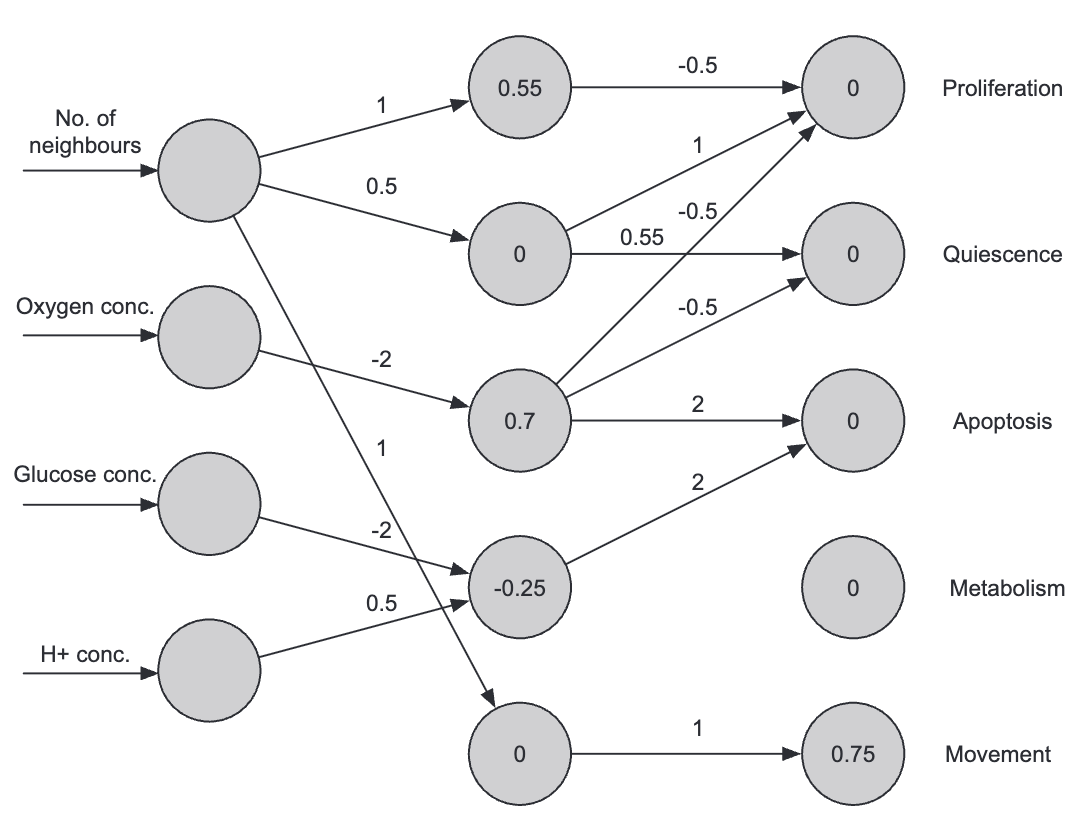
\includegraphics[width=0.96\textwidth,height=0.80\textheight,keepaspectratio]{ann_achitecture.png}
\end{frame}

% ===== Slide: dynamic system =====
\begin{frame}[c]{Dynamic model as a coupled system}
\small
\begin{block}{Full model formulation}
\[
\begin{cases}
\partial_t c = D_c\Delta c - f_c(s,R),\\
\partial_t g = D_g\Delta g - f_g(s,R),\\
\partial_t h = D_h\Delta h + f_h(s,R),\\
V_j = T\!\left(\sum_k w_{jk}x_k-\theta_j\right),\quad
O_i = T\!\left(\sum_j W_{ij}V_j-\phi_i\right),\\
A_{ij}(t)=\arg\max\{O_P,O_Q,O_A\},\\
s_{ij}(t+\Delta t)=\mathcal{U}\big(s_{ij}(t),A_{ij}(t),\mathcal{N}_{ij}(t),c,g,h\big),\\
\omega_{\text{child}}=\omega_{\text{parent}}+m\odot\xi,
\;m_k\sim\mathrm{Bernoulli}(p),\;\xi_k\sim\mathcal N(0,\sigma^2).
\end{cases}
\]
\end{block}
\begin{alertblock}{Metabolic modulation (paper Eq. 1)}
\[
F(R)=\max\big(k(R-T_r)+1,\,0.25\big).
\]
\end{alertblock}
\end{frame}

% ===== Slide: non-dimensionalization =====
\begin{frame}[c]{Non-dimensionalization}
\small
\begin{block}{Change of variables}
\[
\tilde{x}=\frac{x}{L},\qquad
\tilde{t}=\frac{t}{\tau},\qquad
\tilde{c}=\frac{c}{c_0},\qquad
\tilde{g}=\frac{g}{g_0},\qquad
\tilde{h}=\frac{h}{h_0}.
\]
\end{block}
\begin{block}{Non-dimensional parameters}
\[
\tilde{D}_i=\frac{D_i\tau}{L^2},\qquad
\tilde{r}_c=\frac{\tau n_0 r_c}{c_0},\qquad
\tilde{r}_g=\frac{\tau n_0 r_g}{g_0},\qquad
\tilde{r}_h=\frac{\tau n_0 r_h}{h_0}.
\]
\begin{itemize}
  \item In the paper, simulations are run in these non-dimensional variables.
  \item In our project, parameters such as \texttt{c0}, \texttt{Dc}, \texttt{Dt}, \texttt{d}, \texttt{rc} are used in this normalized setting.
\end{itemize}
\end{block}
\end{frame}

% ===== Slide: paper protocol =====
\begin{frame}[c]{Simulation}
\begin{block}{Protocol}
\begin{itemize}
  \item Lattice of size $N=400$ (initially 4 central cells).
  \item Oxygen concentration levels: $c_0$, $c_0/2.5$, $c_0/10$.
  \item 20 runs with different seeds.
  \item Plots of the results.
\end{itemize}
\end{block}
\begin{block}{Measured outputs}
\begin{itemize}
  \item Total tumour cells (alive + dead).
  \item Invasiveness of the tumour.
  \item Shannon diversity index:
  \[
  H(t)=-\sum_k p_k(t)\log p_k(t).
  \]
  \item Comparison plots between different oxygen levels.
\end{itemize}
\end{block}
\end{frame}

% ===== Slide: paper simulation cycle =====
\begin{frame}[c]{Simulation}
\begin{exampleblock}{Single simulation step}
\centering
\begin{minipage}{0.92\textwidth}
\large
\ttfamily
\begin{tabbing}
\hspace*{1.6em}\=\hspace*{1.6em}\=\kill
while t < T:\\[0.20em]
\>for cell in living\_cells:\\
\>\>n <- cell.count\_neighbors()\\
\>\>c, g, h <- cell.get\_state()\\
\>\>o <- cell.ANN(n, c, g, h)\\
\>\>a <- argmax(o.p, o.a, o.q)\\
\>\>cell.update\_state(a)\\[0.20em]
\>t <- t + dt
\end{tabbing}
\end{minipage}
\end{exampleblock}
\vspace{0.2em}
\centering
\normalsize\textbf{Simulation step:} update all living cells once, then advance time by $\Delta t$.
\end{frame}

% ===== Slide: paper results growth =====
\begin{frame}[c]{Paper results: growth and morphology}
\begin{block}{Observed regimes}
\begin{itemize}
  \item $c_0/10$: early hypoxia and fingered morphology.
  \item $c_0/2.5$: delayed death onset and weaker fingering.
  \item $c_0$: rounder growth with necrotic core + viable rim.
\end{itemize}
\end{block}
\begin{exampleblock}{Reference quantitative scale at $t=100$ (paper discussion)}
\[
N_{c_0}\approx 5\times 10^4,
\qquad
N_{c_0/10}\approx 1\times 10^4.
\]
\end{exampleblock}
\end{frame}


% ===== Project section =====
\section{Project Implementation}

% ===== Slide: implementation overview =====
\begin{frame}[c]{Implementation of the model (\texttt{model.py})}
\small
\begin{block}{Implemented model scope}
\begin{itemize}
  \item Oxygen-only reduced model.
  \item States: \texttt{EMPTY}, \texttt{PROLIFERATING}, \texttt{QUIESCENT}, \texttt{NECROTIC}, \texttt{APOPTOTIC}.
  \item ANN input reduced to $\epsilon=[n_{\text{neighbors}}, c]$.
\end{itemize}
\end{block}
\centering
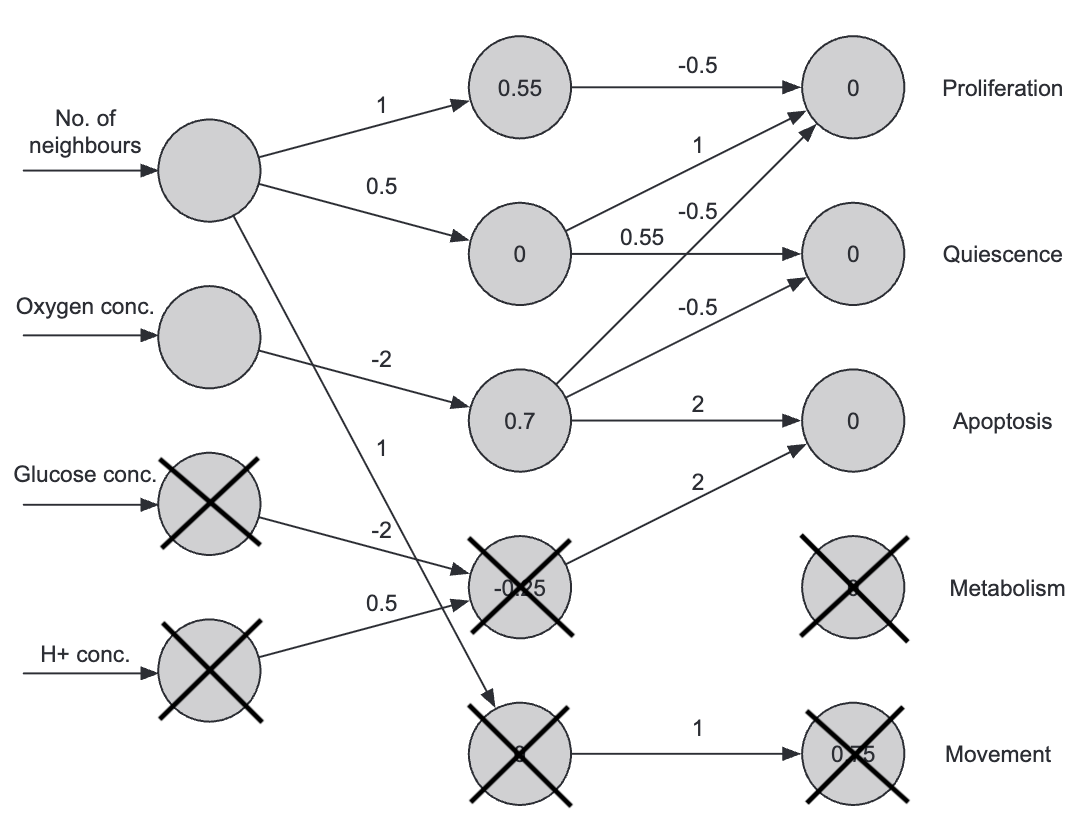
\includegraphics[width=0.85\textwidth,height=0.46\textheight,keepaspectratio]{ann_achitecture_project.png}
\end{frame}

% ===== Slide: implementation diagram =====
\begin{frame}[c]{Implementation diagram}
\centering
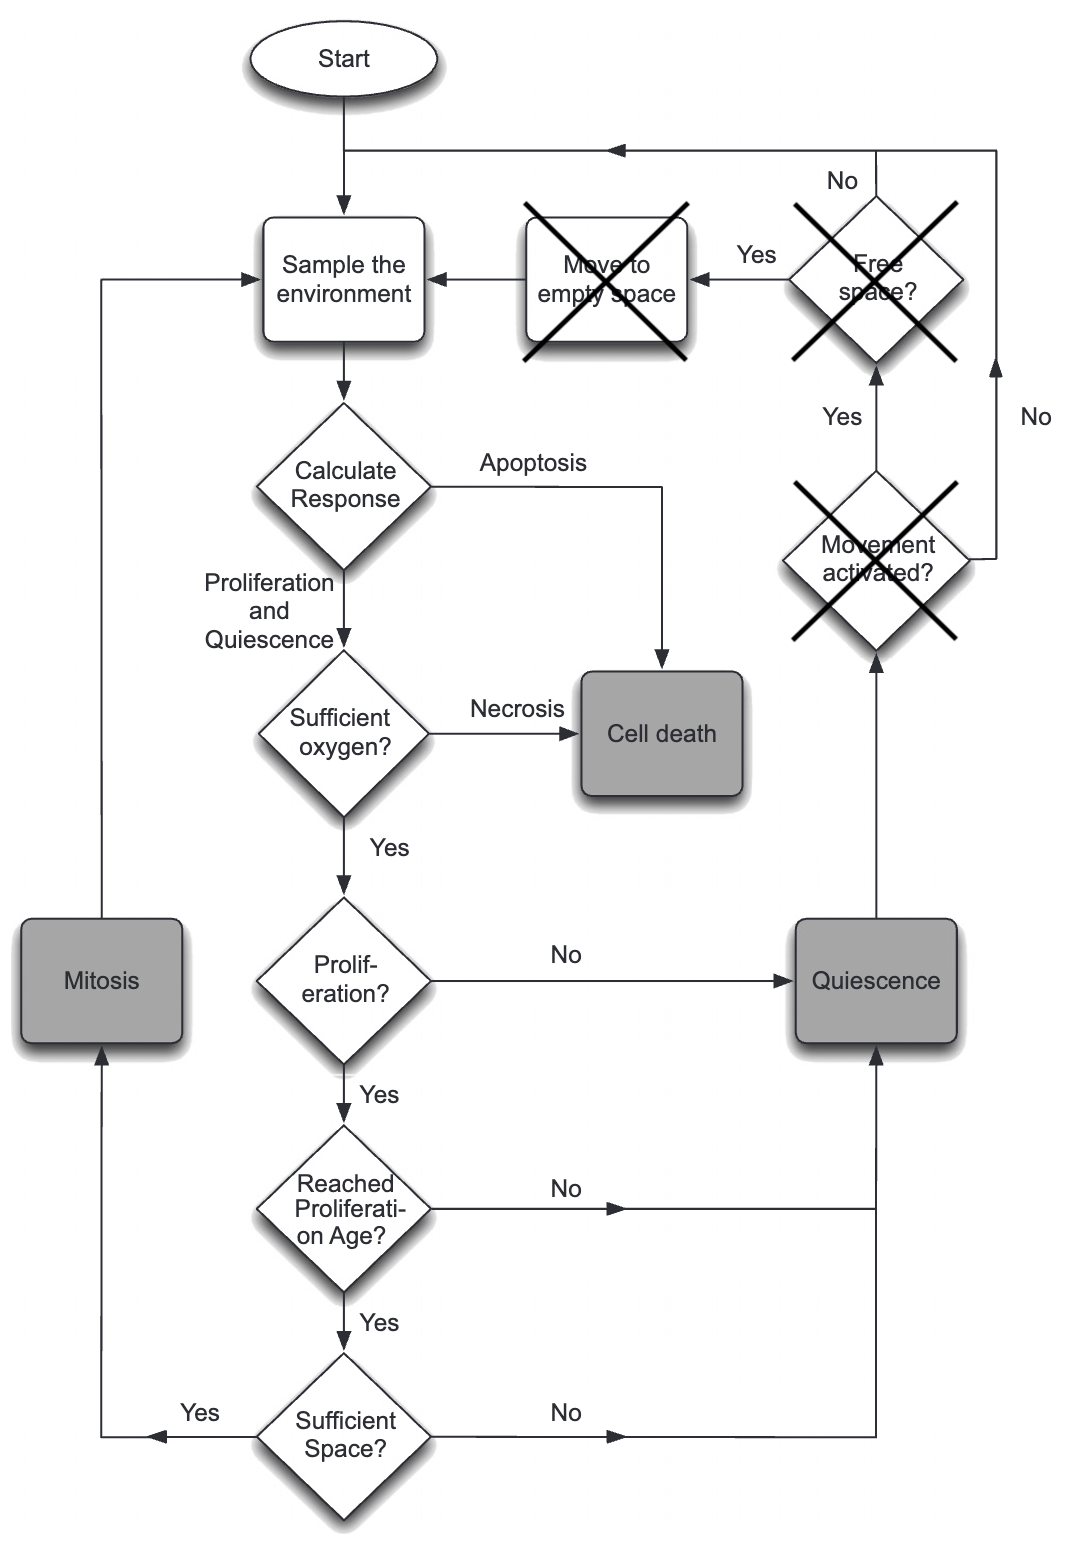
\includegraphics[width=0.96\textwidth,height=0.80\textheight,keepaspectratio]{implementation_diagram_without_movement.png}
\end{frame}

% ===== Slide: default parameters =====
\begin{frame}[c]{Default parameters used}
\tiny
\begin{block}{\texttt{Params} defaults from \texttt{model.py}}
\centering
\begin{tabular}{>{\raggedright\arraybackslash}p{0.32\textwidth}>{\raggedright\arraybackslash}p{0.64\textwidth}}
\toprule
Group & Values \\
\midrule
Lattice/runtime & $N=400$, \texttt{seed\_radius}$=4$, \texttt{steps}$=200$, \texttt{rng\_seed}$=0$ \\
Oxygen field & $c_0=1.0$, $D_c=0.05$, $\Delta t=0.2$, $d=1.0$ \\
Uptake/modulation & $r_c=0.4$, $q=5.0$, $T_r=0.675$, $k=6.0$ \\
Thresholds & $c_{\text{apoptosis}}=0.15$, $n_{\text{quiescence}}=3.0$ \\
Cell cycle & $\Delta t_{\text{age}}=1.0$, $A_p=1.0$, $A_{p,s}=0.5$ \\
Mutation & $p=0.01$, $s=0.25$ \\
\bottomrule
\end{tabular}
\end{block}
\begin{alertblock}{Note}
These defaults are exactly the ones used when notebooks instantiate \texttt{p = Params()}.
\end{alertblock}
\end{frame}

% ===== Slide: ANN training =====
\begin{frame}[c]{ANN implementation and default-weight issue}
\small
\begin{columns}[T,onlytextwidth]
\column{0.56\textwidth}
\begin{block}{\texttt{ann\_training.ipynb} pipeline}
\begin{itemize}
  \item Generate 30k samples from rule labels: A if low oxygen, else P if low crowding, else Q.
  \item Train ANN with mini-batch gradient descent and early stopping.
  \item Save trained parameters to \texttt{.env\_ann\_params}.
\end{itemize}
\end{block}
\begin{block}{Observed issue and fix}
\begin{itemize}
  \item Default ANN (untrained) does not reproduce target policy: accuracy $\approx 0.5404$, recall$_P\approx 0.334$, recall$_A\approx 0.200$.
  \item Trained ANN solves it: accuracy $0.9994$, balanced accuracy $0.9987$, macro F1 $0.9991$, ROC-AUC $1.0000$.
\end{itemize}
\end{block}
\column{0.02\textwidth}
\column{0.40\textwidth}
\centering
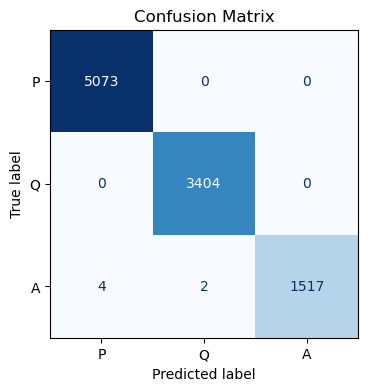
\includegraphics[width=\linewidth,height=0.70\textheight,keepaspectratio]{confusion_matrix.png}
\end{columns}
\end{frame}

% ===== Slide: ANN decision boundary before training =====
\begin{frame}[c]{ANN decision boundary before training}
\centering
\begin{columns}[c,onlytextwidth]
\column{0.50\textwidth}
\centering
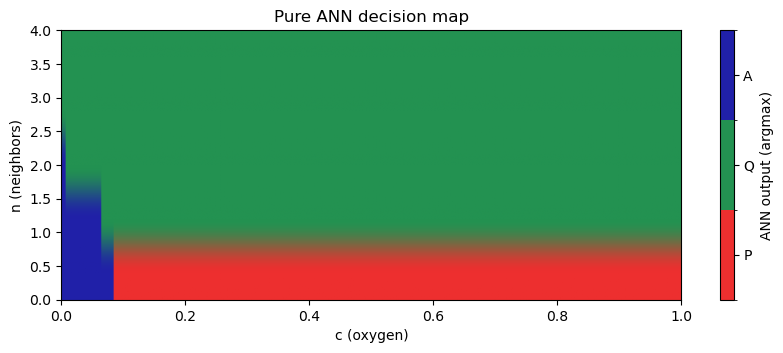
\includegraphics[width=0.98\linewidth,height=0.68\textheight,keepaspectratio]{decision_boundary_pre_training.png}
\vspace{0.15em}
\scriptsize Pre-training ANN map
\column{0.50\textwidth}
\centering
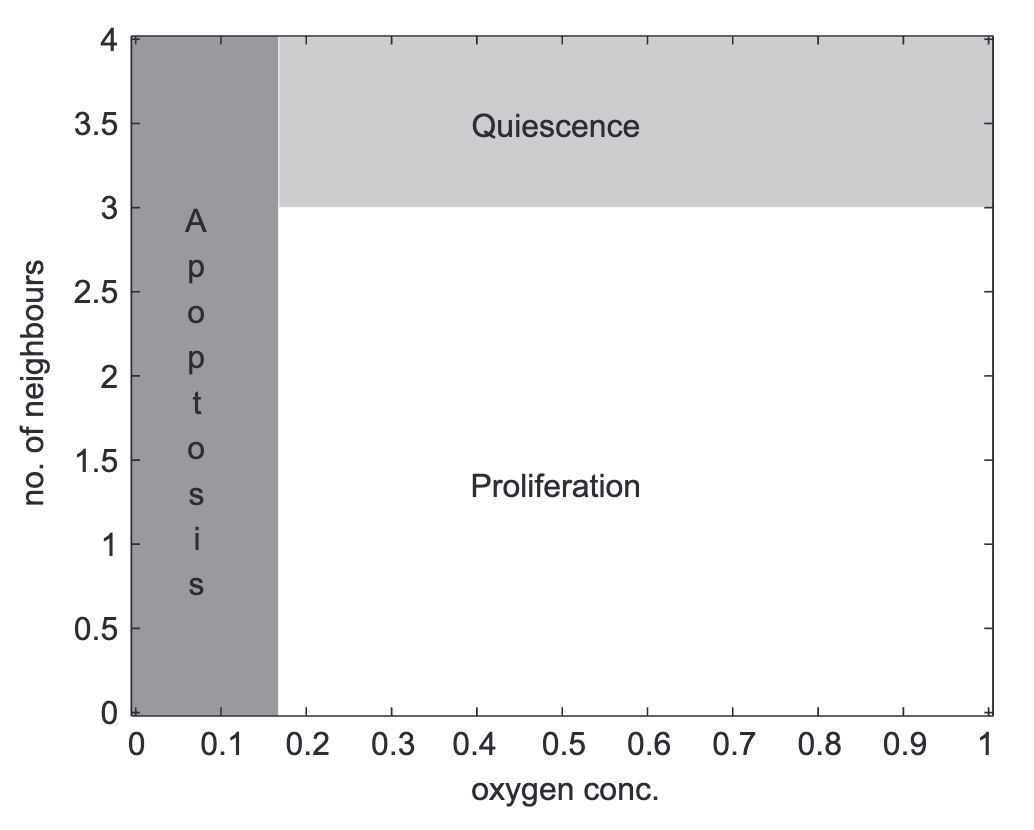
\includegraphics[width=0.98\linewidth,height=0.68\textheight,keepaspectratio]{decision_boundary.png}
\vspace{0.15em}
\scriptsize Reference decision boundary
\end{columns}
\end{frame}

% ===== Slide: ANN decision boundary after training =====
\begin{frame}[c]{ANN decision boundary after training}
\centering
\begin{columns}[c,onlytextwidth]
\column{0.50\textwidth}
\centering
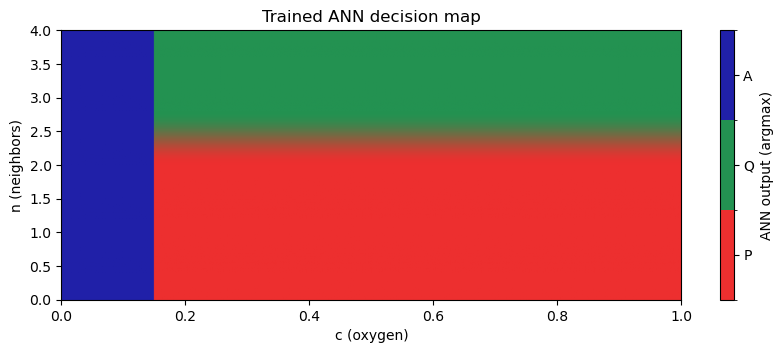
\includegraphics[width=0.98\linewidth,height=0.68\textheight,keepaspectratio]{decision_boundary_post_training.png}
\vspace{0.15em}
\scriptsize Trained ANN map
\column{0.50\textwidth}
\centering
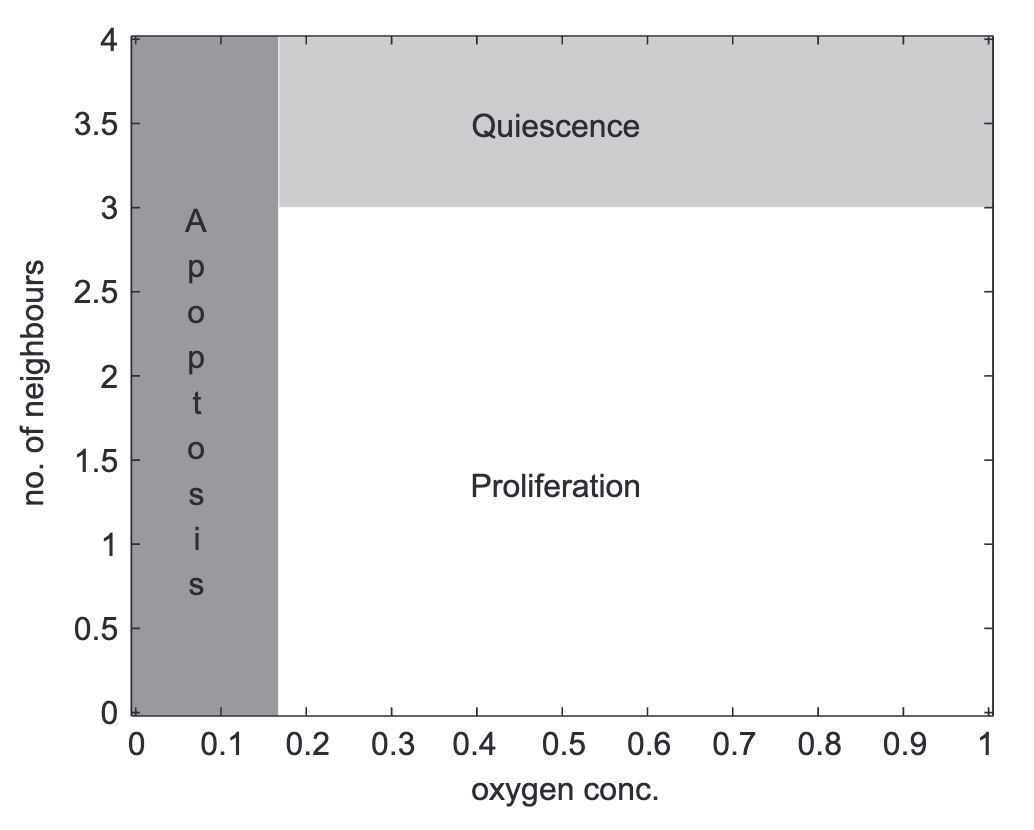
\includegraphics[width=0.98\linewidth,height=0.68\textheight,keepaspectratio]{decision_boundary.png}
\vspace{0.15em}
\scriptsize Reference decision boundary
\end{columns}
\end{frame}

% ===== Slide: multi-seed notebook =====
\begin{frame}[c]{Simulations (\texttt{sim\_over\_multiple\_seed.ipynb})}
\small
\begin{block}{Multi-seed protocol}
\begin{itemize}
  \item Load trained ANN parameters.
  \item Simulate 20 seeds for each oxygen case: $c_0$, $c_0/2.5$, $c_0/10$.
  \item Aggregate trajectories as mean $\pm$ std.
\end{itemize}
\end{block}
\begin{block}{Collected outputs}
\begin{itemize}
  \item Total tumour cells over time.
  \item Invasive distance over time.
  \item Shannon diversity over time.
  \item Summary table at $t=100$.
\end{itemize}
\end{block}
\end{frame}

% ===== Slide: total cells over time =====
\begin{frame}[c]{Population dynamics across oxygen cases (1/2)}
\centering
\begin{columns}[c,onlytextwidth]
\column{0.50\textwidth}
\centering
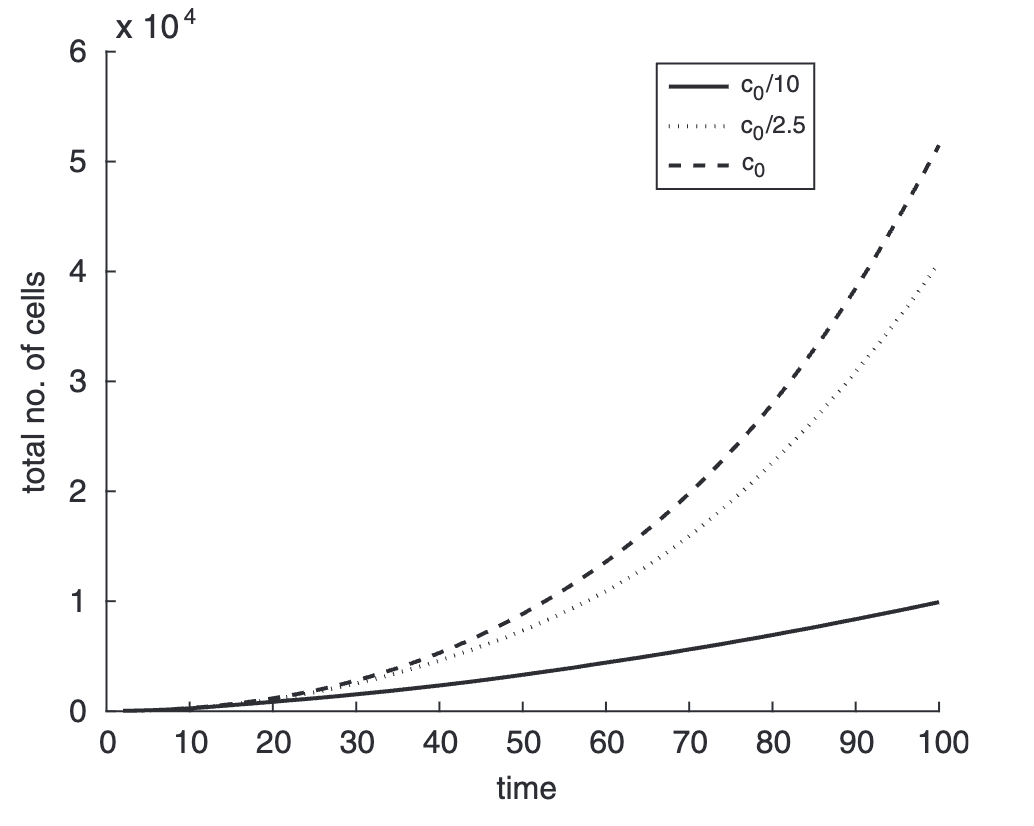
\includegraphics[width=0.98\linewidth,height=0.70\textheight,keepaspectratio]{tot_cells_over_time.png}
\column{0.50\textwidth}
\centering
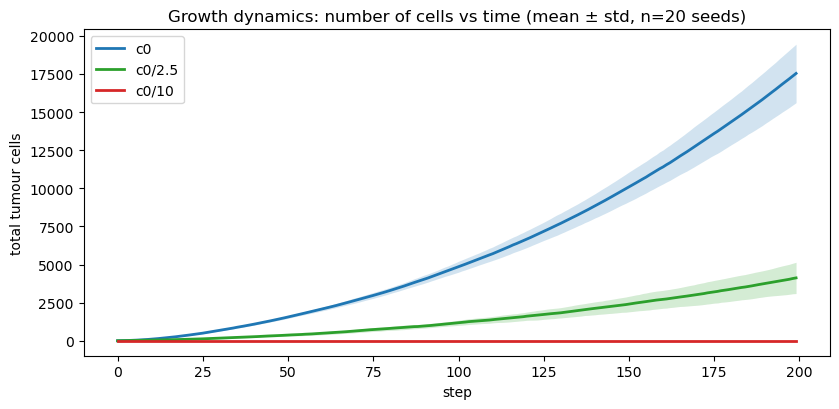
\includegraphics[width=0.98\linewidth,height=0.70\textheight,keepaspectratio]{my_tot_cells_over_time.png}
\end{columns}
\end{frame}

% ===== Slide: population dynamics comparison =====
\begin{frame}[c]{Population dynamics across oxygen cases (2/2)}
\centering
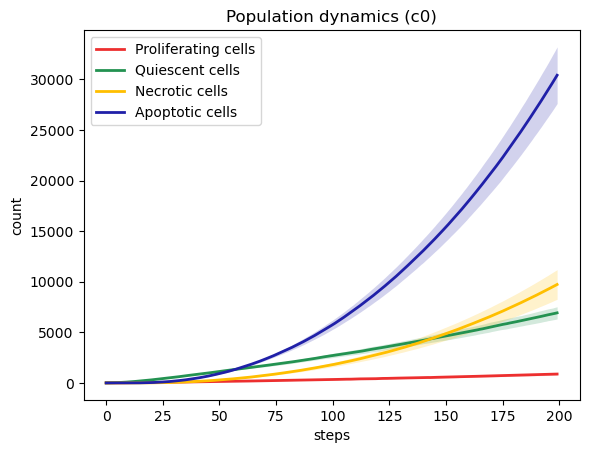
\includegraphics[width=0.315\textwidth]{population_dynamics1.png}\hfill
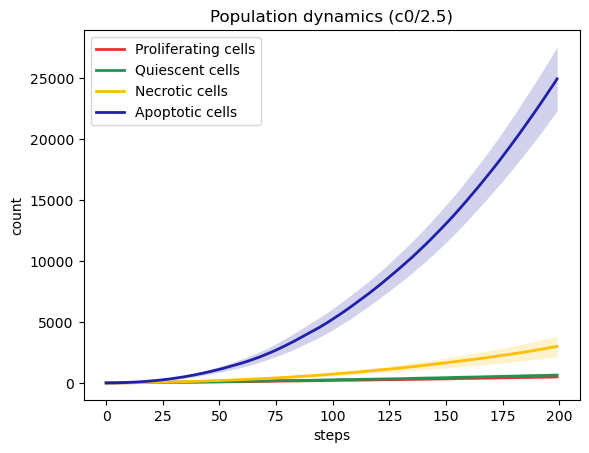
\includegraphics[width=0.315\textwidth]{population_dynamics2.png}\hfill
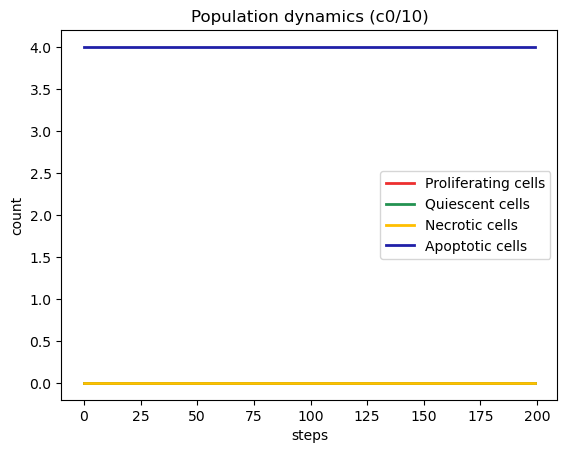
\includegraphics[width=0.315\textwidth]{population_dynamics3.png}
\end{frame}

% ===== Slide: oxygen and necrotic percentage comparison =====
\begin{frame}[c]{Oxygen and necrotic percentage across oxygen cases}
\centering
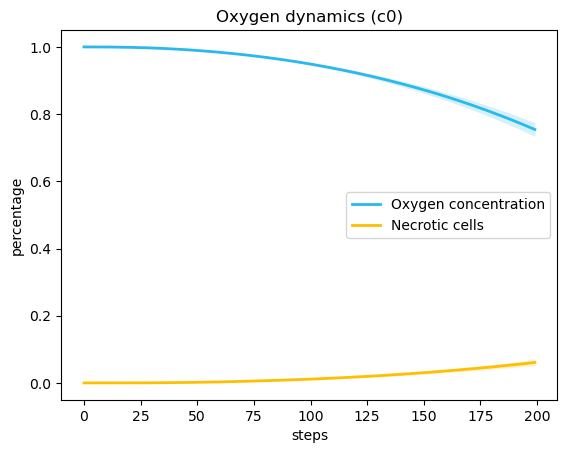
\includegraphics[width=0.315\textwidth]{oxygen_necrotic_pct1.png}\hfill
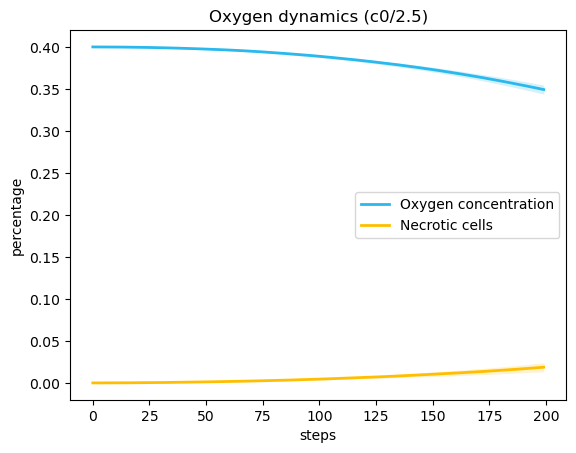
\includegraphics[width=0.315\textwidth]{oxygen_necrotic_pct2.png}\hfill
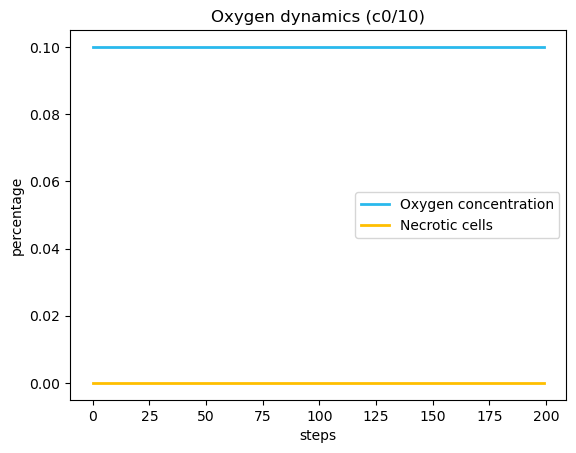
\includegraphics[width=0.315\textwidth]{oxygen_necrotic_pct3.png}
\end{frame}

% ===== Slide: results =====
\begin{frame}[c]{Results}
\small
\begin{block}{Tumour size (mean $\pm$ std)}
\centering
\begin{tabular}{lcc}
\toprule
Oxygen case & Mean tumour size & Std \\
\midrule
$c_0$ & 4772.05 & 340.78 \\
$c_0/2.5$ & 1158.40 & 159.04 \\
$c_0/10$ & 0.00 & 0.00 \\
\bottomrule
\end{tabular}
\end{block}
\begin{exampleblock}{Trend}
\centering
Lower oxygen $\Rightarrow$ lower growth and stronger stress effects.
\end{exampleblock}
\end{frame}

% ===== Slide: differences =====
\begin{frame}[c]{Results}
\small
\begin{block}{What is consistent}
\begin{itemize}
  \item Correct qualitative ordering across oxygen conditions.
  \item Oxygen clearly controls growth/invasion behavior.
\end{itemize}
\end{block}
\begin{alertblock}{What differs quantitatively}
\begin{itemize}
  \item Our sizes are smaller (e.g., $\sim 4.8\times10^3$ vs paper $\sim 5\times10^4$ at $t=100$, $c_0$ case).
  \item In our setup, $c_0/10$ collapses to zero by $t=100$.
\end{itemize}
\end{alertblock}
\begin{block}{Main reasons}
\begin{itemize}
  \item Reduced oxygen-only subsystem and simplified ANN I/O.
  \item Different calibration of uptake, age, and effective time-scale.
  \item Stricter starvation dynamics in our step-wise update.
\end{itemize}
\end{block}
\end{frame}

% ===== Slide: conclusions =====
\begin{frame}[c]{Conclusions}
\begin{block}{Paper side}
\begin{itemize}
  \item Hybrid CA-PDE framework explains oxygen-driven morphology and selection.
\end{itemize}
\end{block}
\begin{block}{Implementation side}
\begin{itemize}
  \item Reproducible implementation with trained ANN and multi-seed analysis.
  \item Qualitative agreement achieved; quantitative calibration remains open.
\end{itemize}
\end{block}
\end{frame}

% ===== References slide =====
\begin{frame}[c]{References}
\small
\begin{itemize}
  \item P. Gerlee, A.R.A. Anderson (2007), \emph{An evolutionary hybrid cellular automaton model of solid tumour growth}, Journal of Theoretical Biology 246:583--603.
  \item Project files: \texttt{simulation/model.py}, \texttt{simulation/ann\_training.ipynb}, \texttt{simulation/sim\_over\_multiple\_seed.ipynb}, \texttt{simulation/utils.py}.
\end{itemize}
\end{frame}

\end{document}
